%!TEX root=../../main.tex

\chapter{Inference for numerical data}
\label{inferenceForNumericalData}

\begin{comment}
	
	-- Go back to chapter 4 to emphasize the possible use of software to compute normal probabilities.
	
	-- Do the same thing here when discussing computing t probabilities
	
\end{comment}


Chapter~\ref{foundationsForInference} introduced some of the primary tools of statistical inference -- point and confidence  interval estimates and hypothesis tests.  This chapter examines some scientific settings where these tools are often used, including the analysis of paired observations and comparing two or more independent groups.  The beginning of the chapter returns to the problem of inference for a population mean, adding a new distribution, the $t$-distribution, which can often be used in small samples. 


%__________________
\section{Inference for one-sample means with the $t$-distribution}
\label{oneSampleMeansWithTDistribution}


The tools studied in Chapter~\ref{foundationsForInference} all made use of the $t$-statistic from a sample mean:
\[
   t = \frac{\overline{x} - \mu}{s}.
\]
The parameter $\mu$ was a population mean, and $\overline{x}$ and $s$ were the sample mean and standard deviation.  Tests and confidence intervals were restricted to samples of at least 30 independent observations from a population where there was no evidence of strong skewness.  This restriction justified appealing to the Central Limit Theorem to calculate probabilities for the $t$-statistic from the normal probability model. If the data are approximately symmetric and there are no large outliers, the $t$-statistic has what is called a $t$-distribution in sample sizes smaller than 30.  That is where the $t-$statistic gets its name.  Using the normal distribution as the sampling distribution of the $t$-statistic essentially treats $s$ as a good replacement for the unknown population standard deviation, $\sigma$.  The sample standard deviation $s$ is really an estimate of $\sigma$, and has an inherent variability just as $\overline{x}$ does.  The $t$ density function has a shape  similar to the normal density but adjusts for the variability in $s$ by having more probability in the left and right tails -- it has more variability.


\subsection{The $t$-distribution}
\label{introducingTheTDistribution}

\index{t-distribution|(}
\index{distribution!$t$|(}

A $t$-distribution, shown as a solid line in Figure~\ref{tDistCompareToNormalDist}, has a bell shape. However, its tails are thicker than the normal model's. This means observations are more likely to fall beyond two standard deviations from the mean than under the normal distribution.\footnote{The standard deviation of the $t$-distribution is actually a little more than 1. However, it is useful to always think of the $t$-distribution as having a standard deviation of 1 in all of our applications.} While our estimate of the standard error will be a little less accurate when we are analyzing a small data set, the extra thick tails of the $t$-distribution correct for the variability in $s$. 

\begin{figure}
\centering
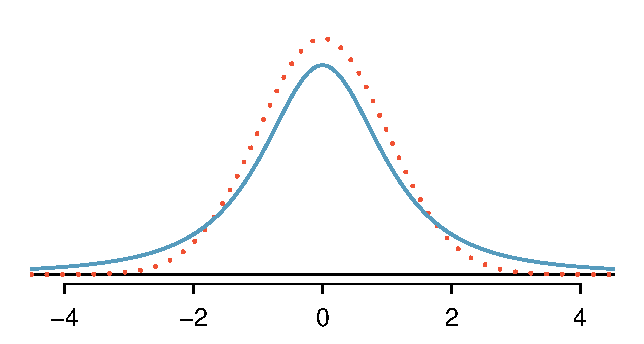
\includegraphics[height=45mm]{ch_inference_for_means_oi_biostat/figures/tDistCompareToNormalDist/tDistCompareToNormalDist}
\caption{Comparison of a $t$-distribution (solid line) and a normal distribution (dotted line).}
\label{tDistCompareToNormalDist}
\end{figure}

The $t$-distribution, always centered at zero, has a single parameter: degrees of freedom.  Several $t$-distributions are shown in Figure~\ref{tDistConvergeToNormalDist}. When there are more degrees of freedom, the $t$-distribution looks very much like the standard normal distribution.

\begin{figure}
\centering
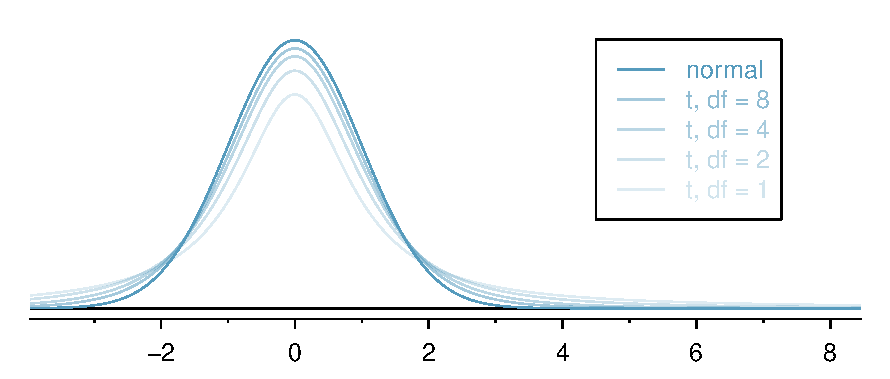
\includegraphics[width=0.8\textwidth]{ch_inference_for_means_oi_biostat/figures/tDistConvergeToNormalDist/tDistConvergeToNormalDist}
\caption{The larger the degrees of freedom, the more closely the $t$-distribution resembles the standard normal model.}
\label{tDistConvergeToNormalDist}
\end{figure}

\begin{termBox}{\tBoxTitle{Degrees of freedom (df)}
The degrees of freedom describe the shape of the $t$-distribution. The larger the degrees of freedom, the more closely the distribution approximates the normal model.}
\end{termBox}

With degrees of freedom of 30 or more, the $t$-distribution is nearly indistinguishable from the normal distribution. The degrees of freedom for the The $t$-statistic in Chapter~\ref{foundationsForInference} has a $t$ distribution with degrees of freedom equal to the sample size - 1, justifying the use of the normal distribution in that chapter.  Section~\ref{tDistSolutionToSEProblem} provides a more complete account of the link between degrees of freedom and sample size.

Probabilities for the $t$-distribution can be calculated using tables of the distribution or using software.  The use of software has become the preferred method because it is more accurate than tables, is not limited to a small range of degrees of freedom and allows complete flexibility in the choice of $t$ values on the horizontal axis.  But each software package uses slightly different commands, so this section illustrates the use of a \term{t-table}, partially shown in Table~\ref{tTableSample}, in place of the normal probability table. A larger $t$-table is in Appendix~\ref{tDistributionTable} on page~\pageref{tDistributionTable}.

\begin{table}[hht]
\centering
\begin{tabular}{r | rrr rr}
one tail & \hspace{1.5mm}  0.100 & \hspace{1.5mm} 0.050 & \hspace{1.5mm} 0.025 & \hspace{1.5mm} 0.010 & \hspace{1.5mm} 0.005  \\
two tails & 0.200 & 0.100 & 0.050 & 0.020 & 0.010 \\
\hline
{$df$} \hfill 1  &  {\normalsize  3.08} & {\normalsize  6.31} & {\normalsize 12.71} & {\normalsize 31.82} & {\normalsize 63.66}  \\ 
2  &  {\normalsize  1.89} & {\normalsize  2.92} & {\normalsize  4.30} & {\normalsize  6.96} & {\normalsize  9.92}  \\ 
3  &  {\normalsize  1.64} & {\normalsize  2.35} & {\normalsize  3.18} & {\normalsize  4.54} & {\normalsize  5.84}  \\ 
$\vdots$ & $\vdots$ &$\vdots$ &$\vdots$ &$\vdots$ & \\
17  &  {\normalsize  1.33} & {\normalsize  1.74} & {\normalsize  2.11} & {\normalsize  2.57} & {\normalsize  2.90}  \\ 
\highlightO{18}  &  \highlightO{\normalsize  1.33} & \highlightO{\normalsize  1.73} & \highlightO{\normalsize  2.10} & \highlightO{\normalsize  2.55} & \highlightO{\normalsize  2.88}  \\ 
19  &  {\normalsize  1.33} & {\normalsize  1.73} & {\normalsize  2.09} & {\normalsize  2.54} & {\normalsize  2.86}  \\ 
20  &  {\normalsize  1.33} & {\normalsize  1.72} & {\normalsize  2.09} & {\normalsize  2.53} & {\normalsize  2.85}  \\ 
$\vdots$ & $\vdots$ &$\vdots$ &$\vdots$ &$\vdots$ & \\
400  &  {\normalsize  1.28} & {\normalsize  1.65} & {\normalsize  1.97} & {\normalsize  2.34} & {\normalsize  2.59}  \\ 
500  &  {\normalsize  1.28} & {\normalsize  1.65} & {\normalsize  1.96} & {\normalsize  2.33} & {\normalsize  2.59}  \\ 
$\infty$  &  {\normalsize  1.28} & {\normalsize  1.64} & {\normalsize  1.96} & {\normalsize  2.33} & {\normalsize  2.58}  \\ 
\end{tabular}
\caption{An abbreviated look at the $t$-table. Each row represents a different $t$-distribution. The columns describe the cutoffs for specific tail areas. The row with $df=18$ has been \highlightO{highlighted}.}
\label{tTableSample}
\end{table}

Each row in the $t$-table represents a $t$-distribution with different degrees of freedom. The columns correspond to tail probabilities. For instance, for a  $t$-distribution with $df=18$, row 18 is used (highlighted in Table~\ref{tTableSample}). The value in this row that identifies the cutoff for an upper tail of 10\% is found in the column where \emph{one tail} is 0.100. This cutoff is 1.33. The the cutoff for the lower 10\% is  -1.33; just like the normal distribution, all $t$-distributions are symmetric.

\begin{example}{What proportion of the $t$-distribution with 18 degrees of freedom falls below -2.10?}
Just like a normal probability problem, we first draw the picture in Figure~\ref{tDistDF18LeftTail2Point10} and shade the area below -2.10. To find this area, we identify the appropriate row: \mbox{$df=18$}. Then we identify the column containing the absolute value of -2.10; it~is the third column. Because we are looking for just one tail, we examine the top line of the table, which shows that a one tail area for a value in the third row corresponds to 0.025. About 2.5\% of the distribution falls below -2.10. In the next example we encounter a case where the exact $t$ value is not listed in the table.
\end{example}

\begin{figure}
\centering
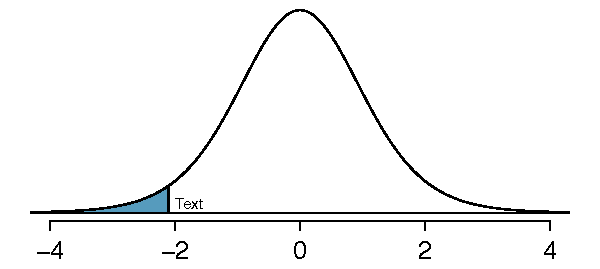
\includegraphics[width=0.5\textwidth]{ch_inference_for_means_oi_biostat/figures/tDistDF18LeftTail2Point10/tDistDF18LeftTail2Point10}
\caption{The $t$-distribution with 18 degrees of freedom. The area below -2.10 has been shaded.}
\label{tDistDF18LeftTail2Point10}
\end{figure}

\begin{example}{A $t$-distribution with 20 degrees of freedom is shown in the left panel of Figure~\ref{tDistDF20RightTail1Point65}. Estimate the proportion of the distribution falling above 1.65.}
We identify the row in the $t$-table using the degrees of freedom: $df=20$. Then we look for 1.65; it is not listed. It falls between the first and second columns. Since these values bound 1.65, their tail areas will bound the tail area corresponding to 1.65. We identify the one tail area of the first and second columns, 0.050 and 0.10, and we conclude that between 5\% and 10\% of the distribution is more than 1.65 standard deviations above the mean. If we like, we can identify the precise area using statistical software: 0.0573.
\end{example}

\begin{figure}
\centering
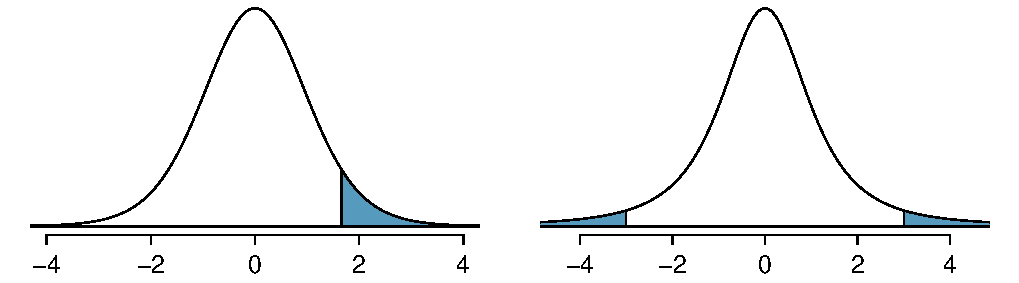
\includegraphics[width=0.85\textwidth]{ch_inference_for_means_oi_biostat/figures/tDistDF20RightTail1Point65/tDistDF20RightTail1Point65}
\caption{Left: The $t$-distribution with 20 degrees of freedom, with the area above 1.65 shaded. Right: The $t$-distribution with 2 degrees of freedom, with the area further than 3 units from 0 shaded.}
\label{tDistDF20RightTail1Point65}
\end{figure}


\subsection{Using the $t$-distribution for tests and confidence intervals for a population mean}
\label{oneSampleTConfidenceIntervalsTests}
\index{data!dolphins and mercury|(}

Chapter~\ref{foundationsForInference} provided formulas for tests and confidence intervals for population means in random samples large enough for the $t$-statistic to have a nearly normal distribution.  In samples smaller than 30 from approximately symmetric distributions without large outliers, the $t$-statistic has a $t$-distribution with degrees of freedom equal to the sample size - 1. Just like inference in larger samples, inference using the $t$-distribution also require that the observations in the sample be independent.  Random samples from very large populations always produce independent observations;  in smaller populations, observations will be approximately independent as long as the size of the sample is no larger than 10\% of the population.

Formulas for tests and intervals using the $t-$distribution are very similar to those using the normal distribution.  For a sample of size $n$ with sample mean $\overline{x}$ and standard deviation $s$, two-sided confidence intervals with confidence coefficient $100(1 - \alpha)$\% have the form
\[
    \overline{x} \pm t_{\text{df}}^{\star}\text{SE},
\]
where 
\begin{itemize}
    
    \item  $\text{SE}= s/\sqrt{n}$ is the standard error of the sample mean;
    
    \item  $t_{\text{df}}^{\star}$ is the point on a $t$-distribution with $n-1$ degrees of freedom and  area $(1 - \alpha/2)$ to its right.
\end{itemize}

A one-sided intervals with the same confidence coefficient will have the form  
\begin{align*}
    \overline{x} &+ t_{\text{df}}^{\star}\text{SE} \text{   (one-sided upper confidence interval)}, \text{  or} \\
    \overline{x} &- t_{\text{df}}^{\star}\text{SE} \text{   (one-sided lower confidence interval)},
\end{align*}
except that in this case $t_{\text{df}}^{\star}$ is the point on a $t$-distribution with $n-1$ degrees of freedom and  area $(1 - \alpha)$ to its right.

\begin{example}{Mercury content in dolphins.}
Dolphins are at the top of the oceanic food chain, which causes dangerous substances such as mercury to concentrate in their organs and muscles. This is an important problem for both dolphins and other animals, like humans, who occasionally eat them. For instance, this is particularly relevant in Japan where school meals have included dolphin at times.
\setlength{\captionwidth}{86mm}

\begin{figure}[h]
\centering
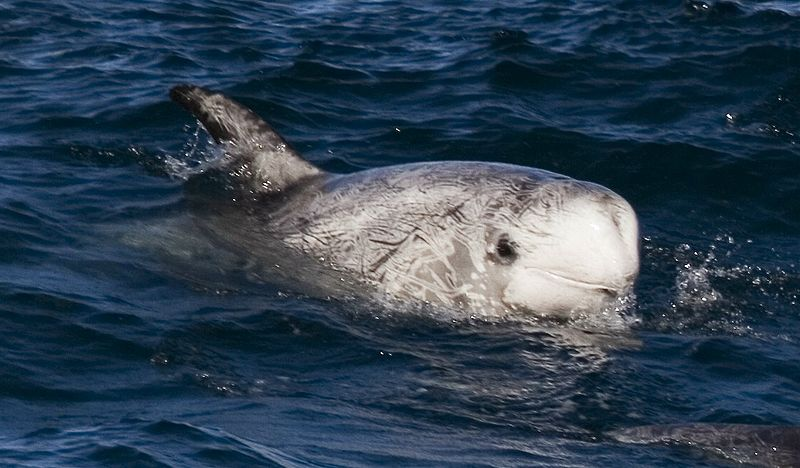
\includegraphics[width=0.8\textwidth]{ch_inference_for_means_oi_biostat/figures/rissosDolphin/rissosDolphin.jpg}  \\
\addvspace{2mm}
\begin{minipage}{\textwidth}
   \caption[rissosDolphinPic]{A Risso's dolphin.\vspace{-1mm} \\
   -----------------------------\vspace{-2mm}\\
   {\footnotesize Photo by Mike Baird (\oiRedirect{textbook-bairdphotos_com}{www.bairdphotos.com}). \oiRedirect{textbook-CC_BY_2}{CC~BY~2.0~license}.}\vspace{-8mm}}
   \label{rissosDolphin}
\end{minipage}
\vspace{3mm}
\end{figure}
\setlength{\captionwidth}{\mycaptionwidth}

This example uses data from a sample of 19 Risso's dolphins from the Taiji area in Japan.\footnote{Taiji was featured in the movie \emph{The Cove}, and it is a significant source of dolphin and whale meat in Japan. Thousands of dolphins pass through the Taiji area annually, and we will assume these 19 dolphins represent a simple random sample from those dolphins. Data reference: Endo T and Haraguchi K. 2009. High mercury levels in hair samples from residents of Taiji, a Japanese whaling town. Marine Pollution Bulletin 60(5):743-747.} The data are summarized in Table~\ref{summaryStatsOfHgInMuscleOfRissosDolphins}. The minimum and maximum observed values can be used to evaluate whether or not there are obvious outliers or skew.

\begin{table}[h]
\centering
\begin{tabular}{ccc cc}
\hline
$n$ & $\overline{x}$ & $s$ & minimum & maximum \\
19   & 4.4	  & 2.3  & 1.7	       & 9.2 \\
\hline
\end{tabular}
\caption{Summary of mercury content in the muscle of 19 Risso's dolphins from the Taiji area. Measurements are in $\mu$g/wet g (micrograms of mercury per wet gram of muscle).}
\label{summaryStatsOfHgInMuscleOfRissosDolphins}
\end{table}

The observations are a simple random sample consisting of less than 10\% of the population, so independence of the observations is reasonable. The summary statistics in Table~\ref{summaryStatsOfHgInMuscleOfRissosDolphins} do not suggest any skew or outliers; all observations are within 2.5 standard deviations of the mean. Based on this evidence, the approximate normality assumption seems reasonable.

With large samples, $z^{\star}$ and the standard error to determine the width of a confidence interval. With a sample size of 19, it will be more accurate to use the $t$-distribution:
\begin{align*}
\overline{x} \pm  t^{\star}_{\text{df}}\text{SE} &= \overline{x}  \pm  t^{\star}_{18} \sqrt{s}/n \\
&= 4.4 \pm  2.10 2.3/\sqrt{19} \\
&= (3.29, 5.51)\,\, \mu\text{g/wet g}.
\end{align*}

The point $z^{\star}$ from a normal distribution is replaced by a point from a $t$-distribution, but sample mean and estimated standard error are unchanged.  In this example the $t^{\star}$ point can be read from the in the $t$-table on page~\pageref{tTableSample}, in the column with area totaling 0.05 in the two tails (third column), the row with 18 degrees of freedom.  Based on these data, one can be 95\% confident the average mercury content of muscles in Risso's dolphins is between 3.29 and 5.51 $\mu$g/wet gram, which is considered high.
\end{example}

The blue fin tuna example in Chapter~\ref{foundationsForInference} cited 0.50 $\mu$g/wet g as the cutoff for safe limits of mercury content.  The two-sided confidence interval for population mean mercury content $
mu$ in the shark muscle example shows that the two-sided hypothesis $H_0: \mu = 0.5$ vs $H_A: \mu > 0.5$ would be rejected at the 0.05 level of significance.  The data provide statistically significant evidence that mercury content in this population is different from 0.1 $\mu$g/wet gram and is, in fact, higher than 0.50.  A formal significance test uses the $t$-statistic
\begin{align*}
	t &= \frac{\overline{x} - \mu_0}{\text{SE}} \\
	  &= \frac{4.4 - 0.50}{2.3/\sqrt{19}} \\
	  &= 7.39.
\end{align*}
Line 18 of the $t$-table on page~\pageref{tTableSample} shows that the probability that the absolute value of a $t$-random variable with 18 df is greater than 7.39 is smaller than 0.01. So for this test, $p < 0.01$, where $p$ is the p-value for the test. Using software, one can show that in fact the $p < 0.001$.

\begin{exercise} \label{croakerWhiteFishPacificExerConditions}
\index{data!white fish and mercury|(}
The FDA's webpage provides some data on mercury content of fish.\footnote{\oiRedirect{textbook-fda_mercury_in_fish_2010}{www.fda.gov/food/foodborneillnesscontaminants/metals/ucm115644.htm}} Based on a sample of 15 croaker white fish (Pacific), a sample mean and standard deviation were computed as 0.287 and 0.069 ppm (parts per million), respectively. The 15 observations ranged from 0.18 to 0.41 ppm. It is reasonable to assume these observations are independent. Based on summary statistics, does the normality assumption seem reasonable? \footnote{There are no obvious outliers; all observations are within 2 standard deviations of the mean. If there is skew, it is not evident. There are no red flags for the normal model based on this (limited) information.}
\end{exercise}

\begin{example}{Estimate the standard error of $\bar{x}=0.287$ ppm using the data summaries in Guided Practice~\ref{croakerWhiteFishPacificExerConditions}. If the $t$-distribution is used to calculte a 90\% confidence interval for the population mean of the mercury content, identify the degrees of freedom and find $t^{\star}_{\text{df}}$.}
\label{croakerWhiteFishPacificExerSEDFTStar}
The standard error: $\text{SE} = \frac{0.069}{\sqrt{15}} = 0.0178$. Degrees of freedom: $\text{df} = n - 1 = 14$.

Using the column where two tails is 0.100 (for a 90\% confidence interval) and row $\text{df}=14$,  $t^{\star}_{14} = 1.76$.
\end{example}

\begin{exercise}
Using the results of Guided Practice~\ref{croakerWhiteFishPacificExerConditions} and Example~\ref{croakerWhiteFishPacificExerSEDFTStar}, compute a 90\% confidence interval for the average mercury content of croaker white fish (Pacific).\footnote{$\bar{x} \ \pm\ t^{\star}_{14} SE \ \to\  0.287 \ \pm\  1.76\times 0.0178\ \to\ (0.256, 0.318)$. We are 90\% confident that the average mercury content of croaker white fish (Pacific) is between 0.256 and 0.318 ppm.}

\index{data!white fish and mercury|)}

\end{exercise}

\section{Paired Data}
\label{pairedData}

\index{paired data|(}


Did a new design for wet suits bring about increased swimming times in the 2000 Olympics? Many people thought so.  de Lucas and co-authors (2000)\footnote{De Lucas et. al, The effects of wetsuits on physiological and biomechanical indices during swimming. \textit{Journal of Science and Medicine in Sport,} 2000; 3(1): 1-8} designed and conducted a study to test the hypothesis that suits had no effect on swimming speed. 

Twelve competitive swimmers swam 1500m at maximum speed, once wearing a wetsuit and once wearing a regular swimsuit, with the order of wetsuit vs swimsuit randomized for each of  the 12 swimmers.  The Investigators recorded maximum velocity for each swimmer, measured in meters per second (m/sec). The data in Table~\ref{swimSuitTimes} can be found in Table 3 the de Lucas paper and in the Lock, et. al. text\footnote{Lock et. al \textit{Statistics, Unlocking the Power of Data}, Wiley, 2013.}

% Tue Jul 26 15:15:14 2016
\begin{table}[ht]
\centering
\begin{tabular}{rrrr}
  \hline
 & swimmer.number & wet.suit.velocity & swim.suit.velocity \\ 
  \hline
1 & 1.00 & 1.57 & 1.49 \\ 
  2 & 2.00 & 1.47 & 1.37 \\ 
  3 & 3.00 & 1.24 & 1.35 \\ 
  4 & 4.00 & 1.35 & 1.27 \\ 
  5 & 5.00 & 1.22 & 1.12 \\ 
  6 & 6.00 & 1.75 & 1.64 \\ 
  7 & 7.00 & 1.64 & 1.59 \\ 
  8 & 8.00 & 1.57 & 1.52 \\ 
  9 & 9.00 & 1.56 & 1.50 \\ 
  10 & 10.00 & 1.53 & 1.45 \\ 
  11 & 11.00 & 1.49 & 1.44 \\ 
  12 & 12.00 & 1.51 & 1.41 \\ 
   \hline
\end{tabular}
\caption{Paired Swim Suit Data} 
\label{swimSuitTimes}
\end{table}

\begin{comment}
wet.suit.velocity = c(1.57, 1.47, 1.24, 1.35, 1.22, 
                      1.75, 1.64, 1.57, 1.56, 1.53, 
                      1.49, 1.51 )
swim.suit.velocity = c(1.49, 1.37, 1.35, 1.27, 1.12, 
                       1.64, 1.59, 1.52, 1.50, 1.45, 
                       1.44, 1.41)
swimmer.number = c(1:12)
swim.suit.study = as.data.frame(cbind(swimmer.number,
                   wet.suit.velocity, 
                   swim.suit.velocity))

swim.suit.study

xtable(swim.suit.study, caption="Paired Swim Suit Data", 
       label="swimSuitTimes")
	
\end{comment}
The swimsuit velocity dataset is an example of \term{paired data} -- each swimmer has two measured velocities, one with a wet suit and one with a regular swimsuit.  A natural measure of the effect of the wet suit is the difference between the measured maximum velocities (\texttt{wet.suit.veocity - swim.suit.velocity}), and the average difference may shed some light on wet suit effect.  The analysis of the differences from these paired measurements uses the $t$-statistic for a confidence interval and test.  Even though there are two measurements per swimmer, the difference in velocities reduces the problem to a one-sample problem, essentially identical in structure to the problems discussed in Section~\ref{oneSampleMeansWithTDistribution}.

Suppose the parameter $\delta$ is the population average of the difference in maximum velocities during a 1500m swim if all competitive swimmers swam with each swim suit type.  This is, of course, a hypothetical population of values, but is useful conceptually in this setting.  When a new intervention is tried for the first time, it is standard practice not to assume that the effect of the intervention will be positive  -- medicine has many examples where new drugs thought to be useful turned out to be harmful.  So in this setting, a natural test to start with is the two-sided $t$-test for the hypothesis
\[
    H_0: \delta = 0 \text{  vs.  } H_A: \delta \neq 0.
\]

The important assumptions behind the test which should not be ignored:
\begin{itemize}
	
	\item  The data are a random sample from the population.  The observations are very likely independent, but it is more difficult to justify the assumption that the sample of swimmers is drawn randomly from the population of competitive swimmers.  The swimmers are a collection of volunteers for this study.  Nevertheless, it is often assumed in problems such as this that the swimmers participating in the study are reasonably representative of competitive swimmers.
	
	\item The population of differences is approximately normally distributed.  This is a small sample, one in which normality would be difficult to confirm.  The dot plot for the difference in velocities is shown in Figure~\ref{swimmerDotPlot} and shows approximate symmetry with no large outliers, so the assumption is probably reasonable.
	
\end{itemize}	

\textit{dotplot goes here}

\begin{comment}
	-- have to give the t-stat
	
	-- conclusions
	
	-- two-sided  confidence interval
	
	-- algebraic formulatio
\end{comment}